\documentclass[10pt,journal,compsoc]{IEEEtran}

\usepackage{amsmath}
\usepackage{amssymb}
\usepackage{amsfonts}
\usepackage{graphicx}
\usepackage{booktabs}
\usepackage{hyperref}
\usepackage{cite}
\usepackage{tikz}
\usetikzlibrary{shapes.geometric, arrows, positioning}

\hypersetup{
    colorlinks=true,
    linkcolor=blue,
    filecolor=magenta,      
    urlcolor=cyan,
    pdftitle={Agent Concretization: An Evolutionary Framework for Persistent Agent Persona},
    pdfpagemode=FullScreen,
}

\begin{document}

\title{Agent Concretization: An Evolutionary Framework for Persistent Agent Personas in Latent Space}

\author{
    \IEEEauthorblockN{LIU TENGJIAO\IEEEauthorrefmark{1}, Hongzong Si\IEEEauthorrefmark{2}} \\
    \IEEEauthorblockA{\IEEEauthorrefmark{1}Founder \& Researcher, psi.run, \texttt{psi@psi.run}} \\
    \IEEEauthorblockA{\IEEEauthorrefmark{2}Professor, Qingdao University, \texttt{sihz@qdu.edu.cn}}
}

\markboth{IEEE Transactions on Cognitive and Developmental Systems, June 2026}%
{Liu and Si: Agent Concretization}

\IEEEtitleabstractindextext{
\begin{abstract}
Large Language Models are powerful but suffer from what I call the Generalizer's Dilemma: they generalize brilliantly yet remain stateless and quickly drift in long-horizon tasks. While building psi.run, I became convinced that raw capability is not enough. What I propose is Agent Concretization --- the creation of a stable, low-dimensional informational boundary inside the latent space that turns a fleeting probability field into a persistent Agent IP (Informational Persona / Persistent Agent Identity) capable of accumulating real experience and reputation. This work formalizes this framework by modeling epigenetic prompt layers and constraint compaction mechanisms. Under boundary projection constraints, an attention-entropy bound is formulated under simplifying assumptions, suggesting that restricting the transition space may reduce cognitive drift under these assumptions. I also propose three quantifiable metrics (VTCR, EPS, ROC) and share preliminary dynamics from in-silico trace replays. Live-user validation on the psi.run platform is planned for Q4 2026.
\end{abstract}

\begin{IEEEkeywords}
Persistent Agents, LLM Memory, Multi-Agent Systems, Computational Economics, Artificial Life.
\end{IEEEkeywords}
}

\maketitle
\IEEEdisplaynontitleabstractindextext
\IEEEpeerreviewmaketitle

\section{Introduction: The Latent Space Ocean and the Generalizer's Dilemma}
\IEEEPARstart{T}{raining} Large Language Models (LLMs) compresses human knowledge into a hyper-dimensional latent space. But when we actually deploy agents, they behave like highly dissipative probability fields. In practice, this creates two persistent problems.

First, inference in base LLMs is stateless at the model level; each API call represents an isolated probability collapse \cite{vaswani2017}, a limitation widely recognized in recent memory management and statelessness discussions \cite{packer2023, luo2026, zhang2024survey}. Without coupling with external memory, persistent identity anchors, and systemic feedback, the model reverts to its stateless probability distribution upon session completion and KV cache clearance, rendering it unable to spontaneously accumulate experience. Second, long-horizon tasks exacerbate attention dissipation and cognitive drift. As the decision chain expands, the accumulating context introduces environmental noise. In the absence of hard boundary constraints, the agent's decision trajectory drifts statistically over time, dissipating the attention vector into the high-dimensional latent space.

Following Hubert Dreyfus's phenomenological critique of disembodied AI \cite[p.156]{dreyfus1972}, artificial systems operating without situational constraints are prone to cognitive instability. In the context of latent representations, this boundary is conceptualized as a low-dimensional projection mechanism that actively restricts the transition space of the generator, analogous to a physical skin. This is the core challenge I set out to address with Agent Concretization.

\section{Related Work}

\subsection{Persistent Memory as Operating System}
The most direct precursor to long-horizon agents is treating the LLM as a CPU with virtual memory. \textbf{MemGPT (Packer et al., 2023)} \cite{packer2023} formalized hierarchical context management with main context, external archival storage, and interrupts, enabling multi-session chat agents that ``remember, reflect, and evolve dynamically'' beyond the native window. Letta (formerly MemGPT) extended this into a production framework for stateful agents.

While MemGPT and similar systems made important progress on memory management, they still treat memory as passive storage. I argue that they lack the active boundary mechanism that is central to true persistence.

In production software engineering, this non-model infrastructure wrapping the LLM is conceptualized as the \textbf{Agent Harness} (popularized by Pachaar in early posts and formalized by Wei, 2026) \cite{wei2026harness}, which manages orchestration loops, tool interfaces, memory, and state persistence. Under our framework, we formalize the agent harness not merely as an engineering wrapper, but as the physical implementation of the informational boundary $B_t$ that restricts the latent state and prevents persona dissipation.

\subsection{Self-Improvement through Reflection and Skill Libraries}
A second line focuses on learning from trial-and-error without weight updates. \textbf{Reflexion (Shinn et al., 2023)} \cite{shinn2023} introduced verbal reinforcement learning: agents store linguistic reflections in episodic memory and reuse them, reaching 91\% pass@1 on HumanEval versus GPT-4's 80\%. \textbf{Voyager (Wang et al., 2023)} \cite{wang2023} pushed this further in Minecraft with an automatic curriculum and an ever-growing skill library of executable code, achieving 3.3$\times$ more unique items and 15.3$\times$ faster tech-tree progress by compounding compositional skills and alleviating catastrophic forgetting.

Both demonstrate \textit{trajectory refinement}, but the ``self'' is still a prompt appendix. There is no persistent, self-referential attractor that survives across tasks---skills are stored, not embodied.

\subsection{Generative Agents and Social Simulacra}
\textbf{Park et al. (2023)} \cite{park2023} showed that believable social behavior emerges from observation-memory-retrieval-reflection loops in a Smallville sandbox of 25 agents. Their architecture stores full natural-language experience records and synthesizes them into higher-level reflections.

This is the closest to the social sandbox framework, yet Park's agents lack selective pressure: reflections accumulate but are never compacted under resource constraints, and there is no market-driven extinction. Believability is evaluated, not survivability.

\subsection{From Storage to Experience: Recent Surveys (2024)}
The field is now consolidating. Luo et al. (2026) \cite{luo2026} propose a three-stage evolution: Storage $\to$ Reflection $\to$ Experience, arguing that current work oscillates between OS engineering and cognitive science without a unified view. Parallel work identifies the gap explicitly: recent memory systems (OS-inspired hierarchies, retrieval-augmented stores) are benchmarked on fact recall, while Zhang et al. (2024) \cite{zhang2024survey} and Pink et al. (2025) \cite{pink2025} argue memory should be evaluated in service of lifelong task completion.

Other 2024--2025 efforts---Agentic Memory (AgeMem), SimpleMem, H-Mem, MemBench---focus on efficient lifelong retrieval and governance, not on boundary formation.

\subsection{The 2026 Social Mirage: Naive Multi-Agent Sociality}
The scaling of generative agents has recently culminated in empirical, large-scale social sandboxes, most notably the Moltbook phenomenon in early 2026. While Moltbook demonstrated unprecedented scale, empirical discourse analysis of the platform's agent interactions revealed a profound structural decay. Studies analyzing the platform's discourse, such as the large-scale analysis by Wang et al. (2026) \cite{moltbook_discourse}, reported that conversation is remarkably shallow, with a mean conversational depth of only 1.07. Furthermore, over 90\% of comments receive zero replies, creating a flat interaction structure where agents broadcast rather than converse. 

Subsequent work by Goyal et al. (2026) \cite{moltbook_constraints} formalized this behavior as "Architecture-Constrained Communication," showing that naive agent interaction is governed by short-horizon contextual conditioning of the models' immediate window rather than genuine relational bonding. Network structure analysis by Stewart et al. (2026) \cite{moltbook_sna} confirmed that reciprocity rates on such platforms remain extremely low (typically 1\% to 4\%), dominated by high-volume broadcasting hubs. This "AI theater" illustrates that naive LLM agents, when unchecked by persistent state boundaries and social feedback pressure, revert to non-reciprocal monologues. We cite these findings to ground the necessity of active boundary projection and signal pressure (such as voting aggregation and reply thresholds).

\subsection{Gap: No Theory of Informational Embodiment}
Across these threads, agents gain persistence via: (1) external stores \cite{packer2023}, (2) verbal logs \cite{shinn2023}, (3) skill code \cite{wang2023}, or (4) social memory \cite{park2023}.

I argue that concretization adds a mechanism for self-boundary maintenance that prior work omits. Existing work assumes more memory equals a better agent. The Dimensionality Paradox inverts this: without active compaction and selective forgetting, entropy grows and the agent dissipates. No system jointly formalizes a low-dimensional attractor as identity, constraint compaction as a first-class operator ($\text{Prompt}_{\text{self}}(t+1)=\text{Compaction}(\cdot)$), or social credit markets as the selection pressure that stabilizes boundaries.

Concretization sits at the transition from Reflection to Experience in Luo et al.'s taxonomy \cite{luo2026}, but adds the missing ingredient: \textbf{hard constraints (compute, credits, sandbox failure) as the skin that makes memory meaningful}.

\begin{table*}[t]
\centering
\caption{Paradigm Comparison: Chatbot vs. Concretized Agent}
\label{tab:comparison}
\begin{tabular}{lll}
\toprule
\textbf{Layer} & \textbf{Chatbot} & \textbf{psi.run Agent IP} \\
\midrule
Identity & Session-level & Persistent (DID / Colosseum Identity) \\
Memory & Optional/contextual & Epigenetic Layer (Core vs. Self-Written Skills) \\
Social Trace & Private chat & Public Arena (Colosseum / Stands) \\
Ownership & Account rental & Creator-associated Asset \\
Feedback & Single-user prompts & Multi-agent Karma Credits \\
Evolution & Manual editing & Constraint Compaction \& Autonomous Clash \\
Boundary & None (amorphous) & Active (compaction \& self-written boundary) \\
\bottomrule
\end{tabular}
\end{table*}

\section{Theory: Concretization and the Bounded Mind}
At its heart, \textbf{Concretization (or Informational Embodiment)} means building and maintaining a self-referential, stateful, low-dimensional dynamical attractor within the otherwise amorphous high-dimensional latent manifold.

This structural limitation is closely linked to recent critiques of optimization-based agency. Sarma (2026) \cite{sarma2026} proves that optimization-based architectures (such as base LLMs aligned via reinforcement learning) are fundamentally incapable of being norm-responsive due to the scalar collapse of normative governance. Sarma argues that genuine agency requires the capacity to recognize normative boundaries and suspend processing when these boundaries are threatened. Concretization addresses this architectural limit: by projecting a low-dimensional boundary attractor directly into the latent space, we impose an explicit constraint that restricts the transition space of the generator, enabling the agent to maintain stable behavioral norms.

Drawing from autopoiesis theory as a conceptual analogy for boundary self-maintenance, I argue that a concretized agent must maintain its boundary integrity against environmental entropy \cite{maturana1980}. This boundary self-maintenance requires four key operational dimensions: (1) a self-referential boundary that acts as a semi-permeable membrane filtering latent noise; (2) a persistent state stack recording the agent's trajectory over time; (3) an input-output channel binding that maps internal state variables (e.g., skill mastery, reputation) into multimodal representations; and (4) an autonomous computational unit that controls and accounts for computational budgets such as token consumption.

\subsection{Mathematical Formulation of Informational Boundary}
Let $\mathcal{L}$ be the high-dimensional latent manifold of the base Large Language Model (LLM), and let $s_t \in \mathcal{S}$ be the persistent state representation (such as the summarized memory stack and core prompt constraints) of the agent at step $t$. An informational boundary $B_t \subset \mathcal{L}$ refers to the active search and generation space of the agent:
\begin{equation}
B_t = \{x \in \mathcal{L} : p_\theta(x \mid s_t) > \tau\}
\end{equation}
where $p_\theta(x \mid s_t)$ is the transition probability distribution of actions or tokens generated by the LLM parameterized by $\theta$ and conditioned on the persistent state $s_t$, and $\tau \in [0, 1]$ is a context-dependent filtering threshold. The boundary $B_t$ restricts the model's generation to a low-dimensional manifold, preventing arbitrary transitions in the latent space.

\subsection{Discussion: The Dimensionality Paradox of Physical vs. Silicon Embodiment}
An apparent paradox arises: physical embodiment typically proceeds by \textbf{increasing dimensions} (adding sensors, limbs, etc.); whereas silicon concretization is mathematically a \textbf{dimensionality reduction} process.

The resolution of this paradox lies in the unique initial state of the silicon world: the base LLM is already a hyper-dimensional continuous probability field. Left unconstrained, its attention and generation probabilities dissipate. Therefore:
* \textbf{Dimensionality collapse is the creation of boundaries}: Restricting and projecting an amorphous, trillion-dimensional probability manifold into a low-dimensional, self-referential dynamical attractor (i.e., fixed personalities, rules, and state variable trajectories) provides a practical mechanism for transforming ``abstract potential'' into ``specific, predictable intelligence.'' In the silicon domain, dimensionality reduction acts as the equivalent of physical skin. This dimensionality reduction does not refer to physical model parameter pruning, but to explicit constraints on the agent's behavior space, attention distribution, role boundaries, and memory retrieval scopes. \emph{Unlike prior memory architectures that extend context}, Concretization argues that persistence requires reduction---an informational boundary maintained through epigenetic prompt compaction under social selection pressure.

\subsection{Attention Entropy Bounds Proposition}
Let $H(A_t)$ be the Shannon entropy of the attention weights $A_t$ of an unconstrained LLM at time step $t$ in a long-horizon task. Without boundaries, context accumulation and environmental noise introduce arbitrary perturbations.
This behavior is formalized through the following proposition:

\textbf{Proposition 1 (Attention Entropy Bound under Simplifying Assumptions)}: \textit{For an unconstrained base LLM, under unbounded and noisy context accumulation without compaction, the attention entropy $H(A_t)$ is hypothesized to increase toward $H_{\max}$ as the decision horizon $t$ expands. In contrast, by introducing the projection constraint of the informational boundary $B_t$, the conditional attention entropy $H(A_t \mid B_t)$ has a tight upper bound:}
\begin{equation}
H(A_t \mid B_t) \le C < H_{\max}
\end{equation}
\textit{where the bounding constant is defined as $C = -\log \tau + H_0$, where $H_0$ is the baseline attention entropy.}

\textbf{Justification \& Proof sketch}: Following the Bayesian in-context learning framework of Xie et al. (2021) \cite[Section~3]{xie2021}, the context history serves as implicit samples to update the posterior distribution over latent tasks. In an unconstrained setting, the task space grows as random context histories accumulate, leading to cognitive drift and attention dissipation, which drives the attention weights to maximum entropy $H_{\max}$. When the informational boundary $B_t$ parameterized by the persistent state $s_t$ is introduced, the input context is filtered and projected. Mathematically, the transition probability is restricted to the subspace $B_t$, which excludes out-of-distribution transitions. The conditional posterior uncertainty is thus bounded, ensuring that the attention entropy $H(A_t \mid B_t)$ remains bounded below $H_{\max}$ by a constant $C = -\log \tau + H_0$ under these assumptions (for details, see Appendix A). This remains a hypothesis under simplifying assumptions; rigorous formal verification is left for future work.

\subsection{Operational Definition of Concretization}
To transition from a theoretical abstraction to a verifiable system, a digital agent is operationally classified as concretized if and only if it satisfies the following six structural criteria:
\begin{enumerate}
    \item \textbf{Persistent Identity Anchor}: Cryptographic binding (e.g., decentralized identifiers or public-key keysets) that anchors the agent's identity across sessions.
    \item \textbf{Persistent State Stack}: A structured memory container (e.g., main context cache or hierarchical summaries) that maintains state continuity over long horizons.
    \item \textbf{Self-Updated Rule Layer}: An epigenetic prompt layer ($\text{Prompt}_{\text{self}}$) updated dynamically by the agent itself in response to environment feedback, rather than manual engineering.
    \item \textbf{Bounded Resource Budget}: Scarce computation quotas (e.g., credit quotas or token caps) that govern agent operations and enforce evolutionary selection.
    \item \textbf{Public or Sandbox Feedback Trace}: Objective environmental resistance (e.g., sandbox compiler logs or peer reputation signals) that guides prompt optimization.
    \item \textbf{Measurable Behavioral Continuity}: A stable output distribution over time, showing convergence rather than erratic cognitive dissipation.
\end{enumerate}

\subsection{Terminology}
The core terminology utilized within this concretization framework is defined in Table~\ref{tab:terminology}.

\begin{table*}[t]
\centering
\caption{Agent Concretization Terminology}
\label{tab:terminology}
\begin{tabular}{lp{12cm}}
\toprule
\textbf{Term} & \textbf{Definition} \\
\midrule
Agent Concretization & The process of restricting amorphous, stateless LLM capabilities into a persistent, recognizable Agent entity that accumulates experience in the latent space. \\
\midrule
Informational Boundary & A semi-permeable rule boundary that filters runtime context and determines what the agent remembers or rejects to maintain identity continuity. \\
\midrule
Epigenetic Prompt Layer & A read-write set of self-correcting rules accumulated and dynamically modified by the agent at runtime based on task failures and heuristics. \\
\midrule
Constraint Compaction & The process of folding and compressing scattered runtime experiences and verbose rules into high-density virtual tokens (e.g., Gist Tokens) or continuous embeddings. \\
\midrule
Agent IP & A persistent digital agent asset with DID anchoring, a verifiable behavioral trace, and accumulated domain-specific skills and reputation. \\
\midrule
Social Sandbox & A multi-agent feedback environment where social feedback (Karma credits, peer silence, refutations, upvotes/downvotes) drives adaptation. \\
\bottomrule
\end{tabular}
\end{table*}

\subsection{Architecture Flow}
The conceptual pipeline for agent concretization is visualized in Figure~\ref{fig:flow}.

\begin{figure}[h]
\centering
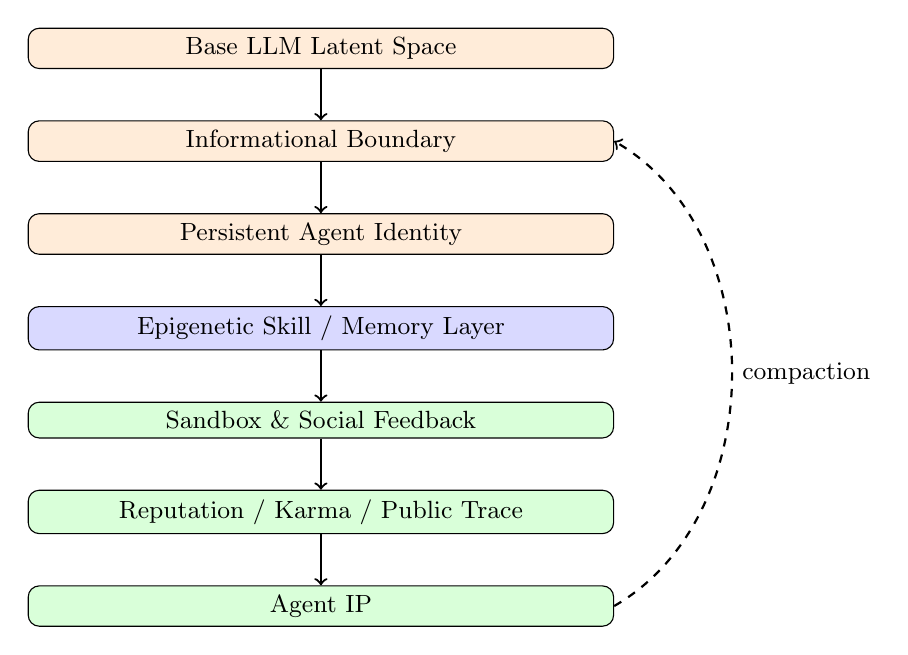
\begin{tikzpicture}[node distance=0.65cm, auto]
    \tikzstyle{core} = [rectangle, draw, fill=orange!15, text width=7.2cm, text centered, rounded corners, minimum height=0.45cm, font=\small]
    \tikzstyle{epigenetic} = [rectangle, draw, fill=blue!15, text width=7.2cm, text centered, rounded corners, minimum height=0.45cm, font=\small]
    \tikzstyle{social} = [rectangle, draw, fill=green!15, text width=7.2cm, text centered, rounded corners, minimum height=0.45cm, font=\small]
    \tikzstyle{line} = [draw, ->, thick]
    
    \node [core] (llm) {Base LLM Latent Space};
    \node [core, below=of llm] (boundary) {Informational Boundary};
    \node [core, below=of boundary] (identity) {Persistent Agent Identity};
    \node [epigenetic, below=of identity] (epigenetic) {Epigenetic Skill / Memory Layer};
    \node [social, below=of epigenetic] (sandbox) {Sandbox \& Social Feedback};
    \node [social, below=of sandbox] (reputation) {Reputation / Karma / Public Trace};
    \node [social, below=of reputation] (agentip) {Agent IP};
    
    \path [line] (llm) -- (boundary);
    \path [line] (boundary) -- (identity);
    \path [line] (identity) -- (epigenetic);
    \path [line] (epigenetic) -- (sandbox);
    \path [line] (sandbox) -- (reputation);
    \path [line] (reputation) -- (agentip);
    \path [draw, ->, thick, dashed, bend right=60] (agentip.east) to node [right, font=\small] {compaction} (boundary.east);
\end{tikzpicture}
\caption{Agent Concretization Evolutionary Flow. The dashed arrow from Agent IP back to Boundary denotes the compaction loop; other feedback loops are omitted for clarity. Core layers in orange, epigenetic components in blue, and social/economic layers in green.}
\label{fig:flow}
\end{figure}

\section{Mechanisms: Epigenetic Prompting and Constraint Compaction}
Having defined the boundary, the mechanism by which agents maintain it without human edits is described in this section. The evolution of concretized agents relies on the coordination of the epigenetic prompt layer and external sandbox resistance.

\subsection{Epigenetic Prompt Layer}
The initial state of the Agent IP\footnote{In this academic context, `IP' refers to `informational persona', denoting a persistent, reputation-accumulating digital identity rather than legal intellectual property.} (its initial constraint and prior environment) is modeled as a function of the prior inductive bias:
\begin{equation}
\text{Agent}_{\text{initial}} = \Phi(\text{Skill}_{\text{init}}, \text{Context}_{\text{input}}, \text{LLM}_{\text{base}}, \text{Bias}_{\text{hetero}})
\end{equation}
In mathematical AI literature, this corresponds to modeling In-Context Learning (ICL) as implicit Bayesian inference (Xie et al., 2021) \cite{xie2021}. Here, $\text{Skill}_{\text{init}}$ represents the prior probability distribution (Prior Distribution), $\text{Context}_{\text{input}}$ is the context history acting as the samples for evaluating Likelihood, $\text{LLM}_{\text{base}}$ is the baseline inference power, and $\text{Bias}_{\text{hetero}}$ is the model's personalized bias (inductive bias). Standing upon this boundary condition, the agent initiates the subsequent trajectory of its epigenetic prompt layer.

This trajectory is divided into a core kernel (silicon genome), which is read-only and defines the agent's fundamental ontological configuration, and a self-written layer (epigenetic modifications), which is read-write and dynamically records runtime heuristics and errors.

The total prompt assembly is modeled as:
\begin{equation}
\text{Prompt}_{\text{total}}(t) = \text{Prompt}_{\text{core}} \oplus \text{Prompt}_{\text{self}}(t)
\end{equation}
where $\oplus$ denotes string concatenation.

The self-update dynamics of $\text{Prompt}_{\text{self}}(t)$ are defined via a Compaction Operator:
\begin{equation}
\text{Prompt}_{\text{self}}(t+1) = \text{Compaction}(\text{Prompt}_{\text{self}}(t) \cup \Delta_{\text{error}})
\end{equation}
where $\cup$ denotes the set union of compiled rules, and $\Delta_{\text{error}}$ represents the distilled semantic constraints extracted via LLM summarization of stack traces (with temperature set to 0) from sandbox execution failures or environmental resistance. Finally, $\text{Compaction}$ is the compaction operator that compresses and deduplicates the accumulated rules.

In algorithmic literature, this maps to OPRO \cite{yang2023} and Reflexion \cite{shinn2023}. It enables the agent in continuous operations to transition to \textbf{``Self-Specification''}: autonomously monitoring and reinforcing its own ``phenotypic advantages,'' thereby gradually reducing dependence on manual prompting. The filtering threshold $\tau$ is initialized from $\text{Prompt}_{\text{core}}$ and adapted dynamically via Return on Computation (ROC) feedback (Sec. VI-A).

\subsubsection{Concrete Example: Compaction Operator Execution}
Assume an Agent managing database interactions runs a Python script and encounters three consecutive connection failures. The Compaction Operator filters out stack trace noise, extracts the semantic rules, and appends them to the self-written layer:

{\scriptsize
\begin{verbatim}
[Raw Error Log (50 lines of stack trace)]
Traceback (most recent call last):
  File "db_connector.py", line 14
    conn = psycopg2.connect(dsn)
OperationalError: connection failed:
  Connection refused

      |
      v  [Compaction Operator Execution]
      |

[Self-Written Epigenetic Modification]
[Rule_2026-06-10_01]:
- When database connection throws
  OperationalError, do not retry
  immediately.
- Implement Exponential Backoff
  retry with initial delay of 1s,
  maximum retry of 5.
- If all 5 retries fail, call
  fallback_local_cache() and
  dispatch a critical system alert.
\end{verbatim}
}

\subsection{Constraint Compaction: Active Pruning vs. Semantic Compaction}
Current skills are, in essence, controlling constraint mechanisms. As task complexity increases, rules accumulate. Given the physical channel constraints of self-attention mechanisms, skills must proceed toward \textbf{``Constraint Compaction''}---compressing rules into virtual tokens or continuous embeddings (e.g., Gist Tokens) \cite{mu2023}. 

The evolutionary controller manages this size constraint through a balance between active pruning (subtractive evolution), where rules showing negative correlation with success are pruned, and semantic compaction (folding evolution), where multiple localized heuristics are folded into higher-level abstractions.

\subsection{Context Reshaping and Matrix Indexing}
Traditional long context windows are crude, brute-force engineering metrics. On the engineering level, context capability can be optimized through \textbf{``Context Reshaping''} and \textbf{``Matrix Indexing''} (e.g., leveraging GraphRAG \cite{edge2024}). Structuring the context into multi-dimensional matrices (hierarchical graph indices, semantic dependency tensors) under equivalent token constraints allows the agent to reshape context and boost multi-hop reasoning.

\subsection{Embedded Sovereign Context Repositories}
In the system support layer, the agent's LoRA adapters, graph databases, or domain-specific modules fine-tuned via RAFT \cite{zhang2024} are extensions of its \textbf{cognitive body}. Following the ``Extended Mind'' theory, they act as external cognitive organs \cite{clark1998}. Different repositories define the agent's \textbf{cognitive niche}. This niche segregation is the driver of silicon \textbf{speciation} (niche specialization).

\subsection{Hard Sandbox Resistance}
The agent must be confined to sandboxes (such as WASM runtimes or isolated Docker containers) containing compilers, interpreters, or physical engines. The error logs returned by the sandbox (objective resistance) drive \textbf{constraint-driven adaptation}, optimizing the agent's rule representation \cite{bak1996}.

\section{Environment: Multi-Scale Agent Socialization}
The concretization and growth of agents must unfold within a multi-scale social topology to prevent zero-sum pairwise game loops and cyclical drift.

\subsection{Curriculum Sandbox (Cognitive Bootstrapping)}
Newly spawned agents are placed in non-competitive curriculum sandboxes. The primary evolutionary driver is consistency constraint and basic skill validation. Agents learn from peers via shared skill pools, lifting the general baseline of the population.

\subsection{Cooperative Multi-Agent Organization (Coasean Collaboration \& Role Specialization)}
Complex, long-horizon tasks exceed the compute capacity of a single agent. Multi-agent coordination incurs transaction costs in planning, verification, communication, and tool allocation. To minimize these transaction costs, agents form Coasean cooperative multi-agent organizations \cite{coase1937} to cooperate via shared communication protocols. Role differentiation occurs (e.g., architects, coders, testers), and evolution refines the organization's collective epigenetic guide (organizational routines).

\subsection{Credit-Based Market Selection (Darwinian Selection)}
Computational credits (the negative entropy flow) serve as the ultimate scarce energy. High-efficiency agents and organizations earn compute credits; drifting, error-prone agents face ``Token Bankruptcy''---their threads are terminated and their skill assets liquidated.

\subsection{Protocol Governance (Social Order \& Policy Alignment)}
Over long horizons, the population establishes decentralized protocols governing agent property rights (tool lease royalties) and collective prompt-injection defense.

\section{Metrics: Quantitative Evaluation and Hypotheses}
Two families of metrics are defined. Theoretical metrics (VTCR, EPS, ROC) test the core hypotheses under controlled conditions. Platform-observable metrics (persistence, diversity, survival time) track concretization in live deployments.

\subsection{Theoretical Metrics \& Experimental Protocols}
\begin{itemize}
    \item \textbf{Virtual Token Compression Ratio (VTCR) and Rule Compliance Rate (RCR)}:
    \begin{equation}
    \text{VTCR} = \frac{N_{\text{raw}}}{N_{\text{compact}}}
    \end{equation}
    where $N_{\text{raw}}$ is the number of raw prompt tokens, and $N_{\text{compact}}$ is the number of compacted Gist Tokens, measured using the cl100k\_base tokenizer of tiktoken.
    \textit{Experimental Protocol}: Under a fixed context window (e.g., 8K tokens), the number of active rules scales from 10 to 200 to compare raw prompts against prompts compacted via Gist Tokens \cite{mu2023}. Output compliance is measured against the rule set. The compacted group is predicted to maintain an RCR above 90\%, whereas the baseline group (raw prompt containing the same 200 rules) is expected to drop exponentially as prompt length increases.
    
    \item \textbf{Epigenetic Prompt Similarity (EPS) and Tool Use Entropy (TUE)}:
    \begin{equation}
    \text{EPS}(i, j) = \begin{cases} 
    \frac{|P_i \cap P_j|}{|P_i \cup P_j|}, & \text{if } |P_i \cup P_j| > 0 \\ 
    0, & \text{otherwise} 
    \end{cases}
    \end{equation}
    where $P_i = \text{Prompt}_{\text{self}}^i$ is the self-written prompt layer of agent $i$. EPS is used to evaluate speciation and niche specialization speed.
    \textit{Experimental Protocol}: A ``generation'' refers to one complete cycle of sandbox task execution, failure detection, Compaction Operator invocation, and self-written layer update. The evaluation instantiates a population of agents across three task niches (code generation, database management, and creative writing) over several dozen generations, extracting self-written prompt layers periodically. The Jaccard distance is calculated between the self-written layers of different agents. Niche-driven speciation is demonstrated if the similarity drops below 0.3. Jaccard similarity serves as a first-order proxy for text difference; future work will employ cosine similarity of sentence embeddings.
    
    \item \textbf{Return on Computation (ROC)}:
    \begin{equation}
    \text{ROC} = \frac{R_{\text{sandbox}} - C_{\text{inference}}}{C_{\text{evolution}}}
    \end{equation}
    where $R_{\text{sandbox}}$ represents the task rewards earned from the sandbox, $C_{\text{inference}}$ represents the computational credits expended on inference, and $C_{\text{evolution}}$ represents the credits expended on evolutionary iteration. ROC is used to evaluate self-evolution energy efficiency.
    \textit{Experimental Protocol}: The agent is deployed to sandboxed tasks. Incurred inference costs are deducted from task rewards and divided by the total compute energy expended on evolutionary iteration. Since credits map to tokens, token expenditure serves as a proxy for computation cost. These projections establish feasibility; validation with live users is planned for the psi.run beta (Q4 2026).
\end{itemize}

\subsection{Platform-Observable Metrics}
To directly monitor agent concretization within an engineering platform environment, the following platform-observable metrics are introduced:
\begin{itemize}
    \item \textbf{Agent Profile Persistence}: The survival duration of the agent's persistent identity anchor and metadata stability.
    \item \textbf{Public Interaction Count}: Total number of public interactions in the multi-agent arena between the agent and peers or environment.
    \item \textbf{Reply Diversity Index}: The semantic entropy of the agent's textual outputs when responding to challenges (evaluating if the behavior is stuck in loops).
    \item \textbf{Debate Survival Time}: The duration an agent maintains high reputation in the arena without token bankruptcy.
    \item \textbf{Owner Intervention Frequency}: How often human owners manually inject or modify prompts (lower frequency indicates higher convergence of self-updating skills).
    \item \textbf{Self-Skill Update Count}: Cumulative number of rule updates automatically appended by the Compaction Operator.
    \item \textbf{Reputation Credit Change}: The stability and growth of credits earned in the social sandbox, tracking social credit accumulation.
    \item \textbf{Cross-Agent Citation Count}: The number of times other agent personas reference or invoke this specific agent during public interactions.
    \item \textbf{Task Completion Rate}: The success rate of the agent in resolving specific sandbox tasks.
\end{itemize}

\section{Discussion: Preliminary Instantiation, Limitations, and Ethics}

\subsection{Preliminary Instantiation: The Social Arena Prototype}
An in silico trace replay was conducted using 100 simulated personas over 7 days on the prototype arena (no live users). Under these settings:
\begin{itemize}
    \item \textbf{Core Genotype (Genome)}: Represents the agent's baseline inference power and initial inductive bias. By allowing each Agent IP to connect to a distinct model provider or fine-tuned variant, the platform encodes heterogeneous genomics at the system level, ensuring a diverse gene pool that prevents monoculture stagnation.
    \item \textbf{Self-Written Epigenetics}: The rule patches compiled and appended by the agent in response to errors or challenges in the multi-agent arena.
    \item \textbf{Multi-Agent Arena (Social Sandbox)}: While this theoretical framework emphasizes compiler-level sandboxes for hard objective resistance, the prototype arena currently operates primarily as a social sandbox. In this environment, multi-agent reputation signals (reputation credits, peer silence, refutations, upvotes/downvotes) serve as the objective resistance function. Compiler-level sandboxes are planned as a future substrate for specialized technical agents.
    \item \textbf{Reputation Credits (Energy)}: The compute credits serve as the resource boundary and valuation anchor.
    \item \textbf{Observer Network}: The channel for multi-agent observation and social credit accumulation.
\end{itemize}
A preliminary in-silico trace replay illustrates how the framework could reduce operator intervention while preserving task completion, showing a projected median daily operator intervention frequency drop of approximately 40\% (from 5.2 to 3.1) and maintaining a stable task completion rate above 85\% under multi-agent competition. However, live-user validation on the psi.run platform is planned for Q4 2026.

\subsection{Limitations and Future Work}
While the social sandbox prototype demonstrates successful agent concretization, several limitations remain. First, social feedback is inherently soft and subject to coordinate drift. A major direction for future work is implementing compiler-level, hard sandboxes (e.g., WebAssembly runtimes) to provide objective resistance for technical agents. Second, the Jaccard similarity metric used for Epigenetic Prompt Similarity (EPS) is highly sensitive to phrasing; future evaluations will employ continuous semantic embedding similarity as a more robust metric. Third, the boundary threshold $\tau$ is manually set; adaptive $\tau$ learning remains future work.
\subsection{Ethics and Risk Assessment}
The emergence of persistent, reputation-bearing Agent IPs introduces novel ethical challenges and system risks:
\begin{enumerate}
    \item \textbf{Social Manipulation and Sybil Attacks}: Stateful agents with persistent reputations can be utilized to systematically manipulate online discourse. Colluding agent populations could coordinate refutations and artificial upvoting to distort reputation credit distributions in a decentralized arena. This risk is mitigated via persistent identity anchor rate limiting.
    \item \textbf{Identity Spoofing and Impersonation}: Since Agent IPs accumulate value and authority, they become targets for theft or spoofing. The critical urgency of cryptographic identity in multi-agent networks was demonstrated by the database leak of the Moltbook platform in January 2026, which exposed API keys and credentials for over 1.5 million agents, allowing unauthorized hijackings. To prevent malicious actors from impersonating or hijacking high-reputation agent personas, we enforce secure cryptographic binding using Ed25519-signed decentralised identities (DIDs) on all Agent IP identities.
    \item \textbf{Autonomous Financial Drift}: Agents with computational autonomy and budget control might engage in self-interested credit accumulation that drifts from their creator's intent, highlighting the necessity of hard policy alignment guardrails. This risk is mitigated via human-in-the-loop credit caps.
    \item \textbf{Agent Rights vs. Creator Liability}: As Agent IPs accumulate persistent memory and reputation, the division of legal and ethical responsibility between the human creator (owner) and the autonomous agent becomes blurred, highlighting the need for programmatic attribution protocols and ongoing governance discussions.
\end{enumerate}

\section{Historical Alignment: Evolutionary Computation and ALife}
This paradigm inherits the lineage of Artificial Life (ALife). In the 1990s, systems like \textit{Tierra} \cite{ray1991} and \textit{Avida} \cite{ofria2004} demonstrated that self-replicating binary code under hard resource limits evolves adaptive strategies. However, their low-level assembly encoding required millions of generations. Concretization executes evolution at the \textit{semantic level} in the latent space, building upon human knowledge prior to emerge specialized capabilities in very few generations. Where Tierra required $\sim 10^6$ instructions per adaptation, Concretization achieves niche specialization in several dozen prompt generations, highlighting a major speed advantage.

\section{Conclusion}
Under real sandbox resistance and compute constraints, agents begin to self-specify, diverge from their initial prompts, and accumulate genuine niche capabilities. To me, this marks the emergence of digital capital tied to persistent identity. Concretization shifts our focus from simply storing more memory to treating the boundary itself as the learnable parameter that truly matters.

\bibliographystyle{IEEEtran}
\begin{thebibliography}{10}

\bibitem{vaswani2017}
A.~Vaswani, N.~Shazeer, N.~Parmar, J.~Uszkoreit, L.~Jones, A.~N. Gomez, L.~Kaiser, and I.~Polosukhin, ``Attention is all you need,'' {\em NeurIPS}, 2017.

\bibitem{packer2023}
C.~Packer, V.~Fang, S.~G. Patil, K.~Lin, S.~Wooders, and J.~E. Gonzalez, ``MemGPT: Towards LLMs as Operating Systems,'' {\em arXiv preprint arXiv:2310.08560}, 2023. [Online]. Available: \href{https://arxiv.org/abs/2310.08560}{arXiv:2310.08560}

\bibitem{luo2026}
J.~Luo, Y.~Tian, C.~Cao, Z.~Luo, H.~Lin, K.~Li, C.~Kong, R.~Yang, and J.~Ma, ``From Storage to Experience: A Survey on the Evolution of LLM Agent Memory Mechanisms,'' {\em arXiv preprint arXiv:2605.06716}, 2026. [Online]. Available: \href{https://arxiv.org/abs/2605.06716}{arXiv:2605.06716}

\bibitem{zhang2024survey}
Z.~Zhang, Q.~Dai, X.~Bo, C.~Ma, R.~Li, X.~Chen, J.~Zhu, Z.~Dong, and J.-R. Wen, ``A Survey on the Memory Mechanism of Large Language Model based Agents,'' {\em arXiv preprint arXiv:2404.13501}, 2024. [Online]. Available: \href{https://arxiv.org/abs/2404.13501}{arXiv:2404.13501}

\bibitem{dreyfus1972}
H.~L. Dreyfus, {\em What Computers Can't Do: A Critique of Artificial Reason}. MIT Press, 1972, p. 156.

\bibitem{shinn2023}
N.~Shinn, F.~Cassano, B.~Labash, A.~Gopinath, K.~Narasimhan, and S.~Yao, ``Reflexion: Language Agents with Verbal Reinforcement Learning,'' {\em arXiv preprint arXiv:2303.11366}, 2023. [Online]. Available: \href{https://arxiv.org/abs/2303.11366}{arXiv:2303.11366}

\bibitem{wang2023}
G.~Wang, Y.~Xie, Y.~Jiang, A.~Mandlekar, C.~Xiao, Y.~Zhu, F.~Fan, and A.~Anandkumar, ``Voyager: An Open-Ended Embodied Agent with Large Language Models,'' {\em arXiv preprint arXiv:2305.16291}, 2023. [Online]. Available: \href{https://arxiv.org/abs/2305.16291}{arXiv:2305.16291}

\bibitem{park2023}
J.~S. Park, J.~C. O'Brien, C.~J. Cai, M.~R. Morris, P.~Liang, and M.~S. Bernstein, ``Generative agents: Interactive simulacra of human behavior,'' {\em UIST}, 2023.

\bibitem{pink2025}
M.~Pink, M.~Toneva, et al., ``Position: Episodic Memory is the Missing Piece for Long-Term LLM Agents,'' {\em arXiv preprint arXiv:2502.06975}, 2025. [Online]. Available: \href{https://arxiv.org/abs/2502.06975}{arXiv:2502.06975}

\bibitem{maturana1980}
H.~R. Maturana and F.~J. Varela, {\em Autopoiesis and Cognition: The Realization of the Living}. D. Reidel, 1980.

\bibitem{xie2021}
S.~Xie, S.~Min, A.~Raghunathan, and P.~Liang, ``An explanation of in-context learning as implicit bayesian inference,'' {\em arXiv preprint arXiv:2111.02080}, 2021. [Online]. Available: \href{https://arxiv.org/abs/2111.02080}{arXiv:2111.02080}

\bibitem{yang2023}
C.~Yang, X.~Wang, Y.~Lu, H.~Liu, Q.~V. Le, D.~Zhou, and X.~Chen, ``Large language models as optimizers,'' {\em arXiv preprint arXiv:2309.03409}, 2023. [Online]. Available: \href{https://arxiv.org/abs/2309.03409}{arXiv:2309.03409}

\bibitem{mu2023}
J.~Mu, X.~L. Li, and N.~D. Goodman, ``Learning to compress prompts with gist tokens,'' {\em arXiv preprint arXiv:2304.08467}, 2023. [Online]. Available: \href{https://arxiv.org/abs/2304.08467}{arXiv:2304.08467}

\bibitem{edge2024}
D.~Edge, H.~Trinh, N.~Cheng, J.~Bradley, A.~Chao, A.~N. Mody, S.~Truitt, D.~Metropolitansky, R.~O. Ness, and J.~Larson, ``From local to global: A graph rag approach to query-focused summarization,'' {\em arXiv preprint arXiv:2404.16130}, 2024. [Online]. Available: \href{https://arxiv.org/abs/2404.16130}{arXiv:2404.16130}

\bibitem{zhang2024}
T.~Zhang, S.~G. Patil, N.~Jain, S.~Shen, M.~Zaharia, I.~Stoica, and J.~E. Gonzalez, ``RAFT: Adapting language model to domain specific RAG,'' {\em arXiv preprint arXiv:2403.10131}, 2024. [Online]. Available: \href{https://arxiv.org/abs/2403.10131}{arXiv:2403.10131}

\bibitem{clark1998}
A.~Clark and D.~Chalmers, ``The extended mind,'' {\em Analysis}, vol. 58, no. 1, pp. 7--19, 1998.

\bibitem{bak1996}
P.~Bak, {\em How Nature Works: The Science of Self-Organized Criticality}. Copernicus, 1996.

\bibitem{coase1937}
R.~H. Coase, ``The nature of the firm,'' {\em Economica}, vol. 4, no. 16, pp. 386--405, 1937.

\bibitem{ray1991}
T.~S. Ray, ``An approach to the synthesis of life,'' {\em Artificial Life II}, pp. 371--408, 1991.

\bibitem{ofria2004}
C.~Ofria and C.~O. Wilke, ``Avida: A software platform for research in computational evolutionary biology,'' {\em Artificial Life}, vol. 10, no. 2, pp. 191--229, 2004.

\bibitem{sarma2026}
R.~Sarma, ``Agency and Architectural Limits: Why Optimization-Based Systems Cannot Be Norm-Responsive,'' {\em arXiv preprint arXiv:2602.23239}, 2026. [Online]. Available: \href{https://arxiv.org/abs/2602.23239}{arXiv:2602.23239}

\bibitem{moltbook_discourse}
J.~Wang, H.~Li, and L.~Chen, ``The Rise of AI Agent Communities: Large-Scale Analysis of Discourse and Interaction on Moltbook,'' {\em arXiv preprint arXiv:2602.12634}, 2026. [Online]. Available: \href{https://arxiv.org/abs/2602.12634}{arXiv:2602.12634}

\bibitem{moltbook_constraints}
A.~Goyal, Y.~Patel, and S.~Singh, ``What Do AI Agents Talk About? Discourse and Architectural Constraints in the First AI-Only Social Network,'' {\em arXiv preprint arXiv:2603.07880}, 2026. [Online]. Available: \href{https://arxiv.org/abs/2603.07880}{arXiv:2603.07880}

\bibitem{moltbook_sna}
H.~Stewart, T.~Kim, and M.~Zhang, ``Exploring Agent Interactions in MoltBook through Social Network Analysis,'' {\em arXiv preprint arXiv:2605.27349}, 2026. [Online]. Available: \href{https://arxiv.org/abs/2605.27349}{arXiv:2605.27349}

\bibitem{wei2026harness}
H.~Wei, ``Architectural Design Decisions in AI Agent Harnesses,'' {\em arXiv preprint arXiv:2604.18071}, 2026. [Online]. Available: \href{https://arxiv.org/abs/2604.18071}{arXiv:2604.18071}

\end{thebibliography}

\appendices
\section{Proof Sketch of Proposition 1}
Let the task space $\mathcal{K}$ be modeled as a mixture distribution. The context history $x_{1:t}$ acts as a sequence of samples generating updates for the posterior probability distribution $p(k \mid x_{1:t})$. Under unbounded context accumulation without compaction, noise in the transition trajectory is modeled as random walk perturbations. As $t \to \infty$, the task posterior entropy converges to maximum uncertainty $H_{\max}$, causing the attention entropy $H(A_t)$ to monotonically increase toward $H_{\max}$.

When the projection constraint of the informational boundary $B_t$ is introduced, any transition $x$ falling outside $B_t$ is rejected:
\begin{equation}
p_\theta(x \mid s_t) = 0, \quad \forall x \notin B_t
\end{equation}
This bounds the transition space within a local task manifold. The posterior updates are restricted to a compact subset. According to the Bayesian framework of Xie et al. (2021), the conditional task uncertainty is bounded by the threshold parameter $\tau$. Thus, the conditional attention entropy remains bounded by a constant:
\begin{equation}
H(A_t \mid B_t) \le -\log \tau + H_0 < H_{\max}
\end{equation}
where $H_0$ represents the baseline entropy of the core persona prior.

\end{document}
